\documentclass[a4paper,12pt]{article}
\usepackage[utf8x]{inputenc}
\usepackage{amssymb}
\usepackage{amsfonts}
\usepackage{mathrsfs}
\usepackage{amsmath}
\usepackage{amsthm}
\usepackage[margin=3cm]{geometry}
\usepackage{times}
\usepackage{graphicx}
\usepackage{dsfont}
\usepackage{enumitem}
\usepackage{fancyhdr} 
\usepackage{hyperref}
\usepackage{setspace}
\usepackage{gensymb}

\pagestyle{fancy}
\fancyhf{}
\lhead{Thomas Delaney}
\rhead{6-Month Review Report}
\cfoot{\thepage}

\newtheorem{theorem}{Theorem}
\newtheorem{proposition}{Proposition}[section]
\newtheorem{lemma}{Lemma}[section]
\newtheorem{corollary}{Corollary}[section]
\theoremstyle{definition}
\newtheorem{definition}{Definition}[section]

\newcommand{\boldnabla}{\mbox{\boldmath$\nabla$}} % to be used in mathmode
\newcommand{\cbar}{\overline{\mathbb{C}}}% to be used in mathmode
\newcommand{\diff}[2]{\frac{d #1}{d #2}}% to be used in mathmode
\newcommand{\difff}[2]{\frac{d^2 #1}{d #2^2}}% to be used in mathmode
\newcommand{\pdiff}[2]{\frac{\partial #1}{\partial #2}} % to be used in mathmode
\newcommand{\pdifff}[2]{\frac{\partial^2 #1}{\partial #2^2}}% to be used in mathmode
\newcommand{\upperth}{$^{\mbox{\footnotesize{th}}}$}%to be used in text mode
\newcommand{\vect}[1]{\mathbf{#1}}% to be used in mathmode
\newcommand{\curl}[1]{\boldnabla \times \vect{#1}} % to be used in mathmode
\newcommand{\divr}[1]{\boldnabla \cdot \vect{#1}} %to be used in mathmode
\newcommand{\modu}[1]{\left| #1 \right|} %to be used in mathmode
\newcommand{\brak}[1]{\left( #1 \right)} % to be used in mathmode
\newcommand{\comm}[2]{\left[ #1 , #2 \right]} %to be used in mathmode
\newcommand{\dop}{\vect{d}} %to be used in mathmode
\newcommand{\cov}{\text{cov}} %to be used in mathmode
\newcommand{\var}{\text{var}} %to be used in mathmode
\newcommand{\mb}{\mathbf} %to be used in mathmode
\newcommand{\bs}{\boldsymbol} %to be used in mathmode
% Title Page
\title{6-Month Review Report}
\author{Thomas Delaney}

\begin{document}

\maketitle
\newpage
\tableofcontents
\newpage

\section{Introduction}
	During the first six months of my PhD program, I have started research in two related topics. The first of those is research into modelling the fluorescence produced by fluorescent calcium indicators. The second is the modelling of responses of large populations of neurons. The calcium modelling will be a short term project to be presented at the British Neuroscience Association conference in April. The data used for the second part of my research will be collected using fluorescent calcium imaging, so the calcium modelling is related. The population modelling research will make up most of the work of my PhD.
	
	I will begin this report by outlining the work I have done on the fluorescence modelling, and then I will move onto the population response modelling. The sections on the fluorescence modelling will firstly give a short description of fluorescent calcium indicators, how they work, and their problems, then I will describe my model that aims to provide a tool for identifying and quantifying these problems, and then I will outline how I plan on finishing up this project.
	
	The section on modelling large populations of neurons will consist of a literature review of the recent developments in this research area followed by an outline of the research that I plan to do for the remainder of my PhD.
	
\section{Modelling fluorescence of calcium indicators}

\subsection{Fluorescent calcium indicators}
	Before fluorescent calcium indicators were invented, the most common way to take readings from more than one neuron was to use electrodes. This involved inserting a tetrode or a number of tetrodes into the brain to measure extra-cellular voltages. These extra-cellular voltage traces were then used to detect action potentials. The strength of the spiking signal, and the position of each tetrode were used by purpose designed algorithms to identify the position of individual neurons and `sort' the spikes, i.e. attribute the spikes to a cell. This method is very good for cell detection, spike detection, and attribution. But inserting tetrodes into the tissue damages the tissue. This can cause cells or connections between cells to be damaged \cite{buzsaki}. Also, the electrodes need to be attached by wires to a device that collects their data. This inhibits the movement of the experimental subject, and makes longitudinal experiments impossible. fMRI can also be used to measure brain activity. But the resolution is no-where near small enough to measure the activity of individual cells.
	
	In order to measure the activity of individual cells, the use of fluorescent calcium indicators within cells was developed. This method has become particularly popular since the invention of two-photon calcium imaging. In this process, a calcium sensitive dye is injected into the body of each cell to be monitored. Or the cells are altered, either by a virus or genetically modified, to make them express a calcium sensitive protein. The dye or the proteins fluoresce when they come into contact with and bind to calcium molecules. Since the firing of an action potential usually involves some influx of calcium molecules, the indicator makes the firing of action potentials observable by photon detection. Two-photon detection allows this method to be used \textit{in vivo} \cite{stosiek}. This allows spike detection without having to damage cells or the connections between them, and enables longitudinal experiments as the subject can survive and move around normally when not being examined. 
	
	\begin{figure}[h]
		\centering
		\begin{tabular}{c}
			(a)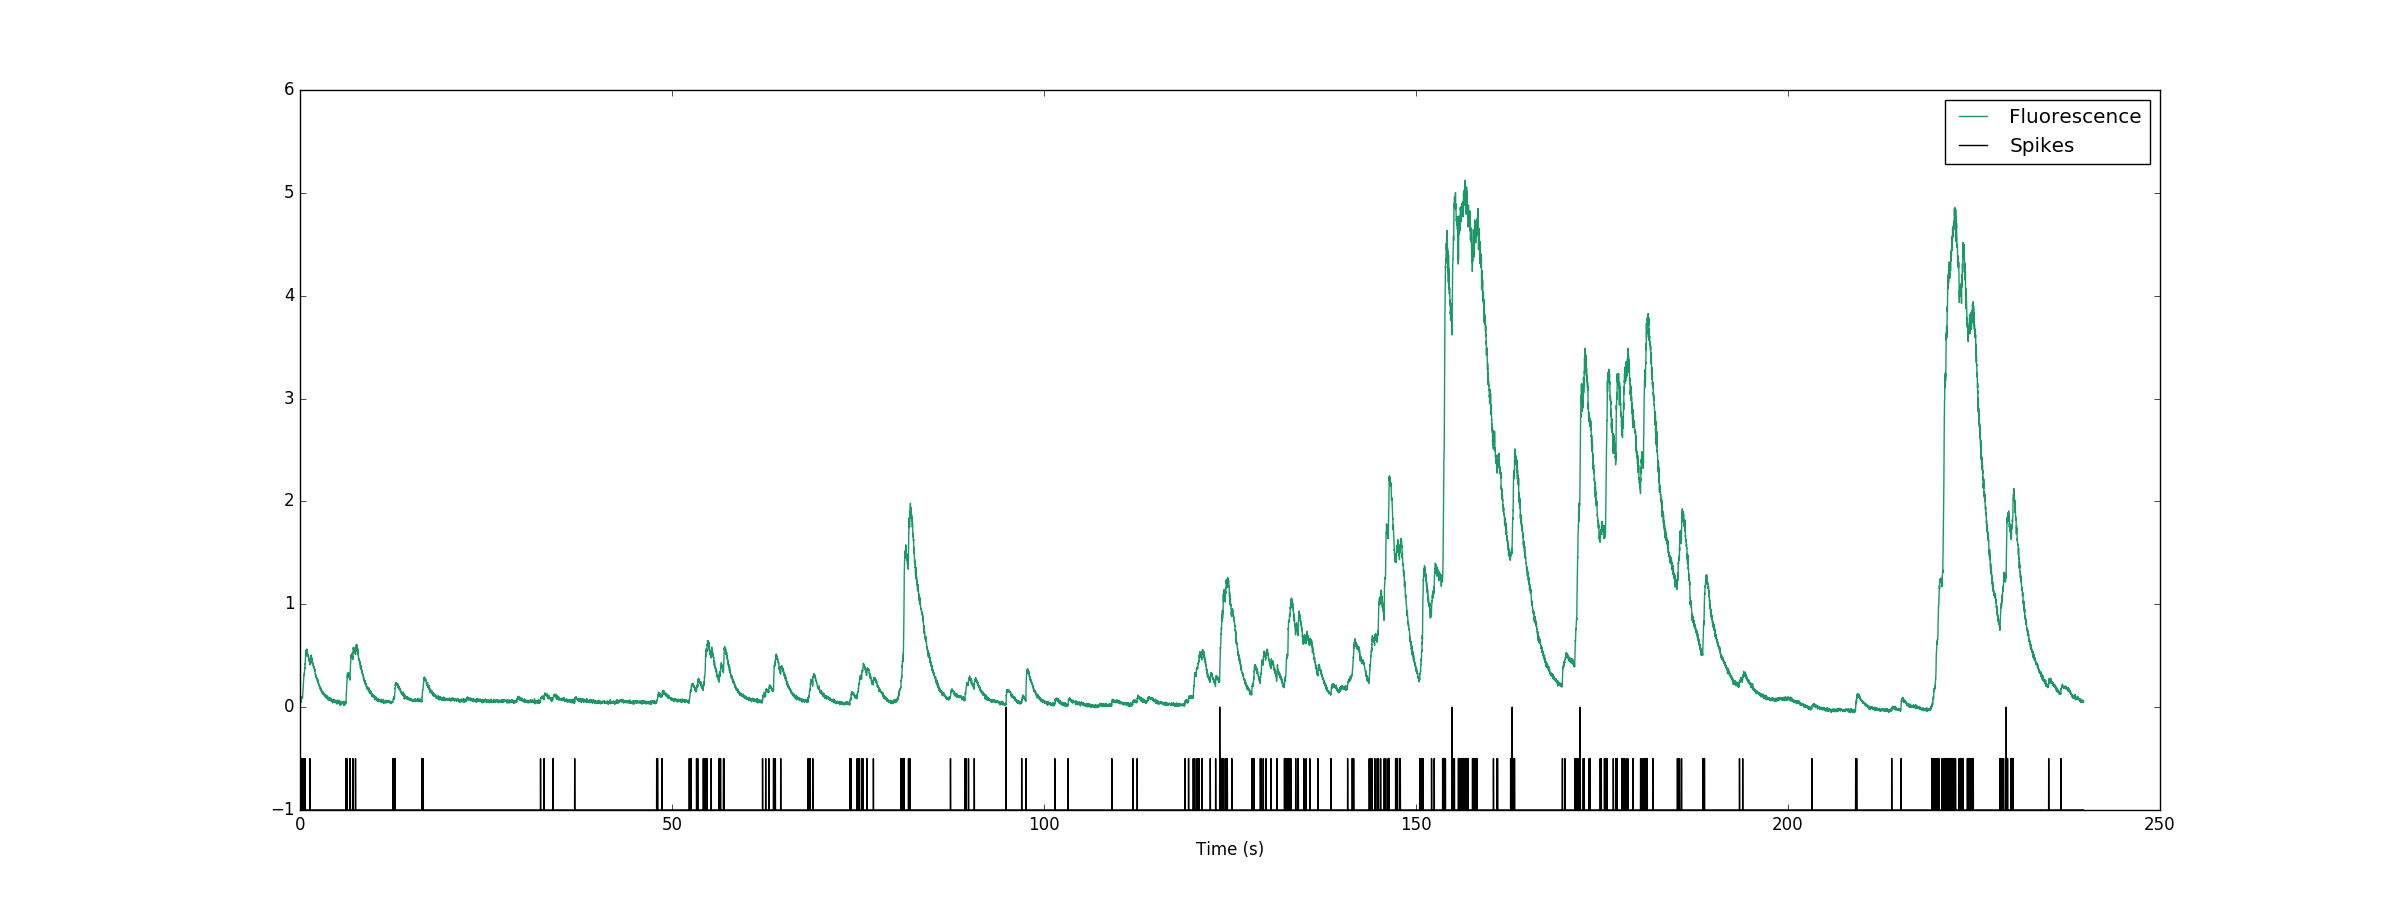
\includegraphics[width=\textwidth]{figures/fluoro_spike_plot_chen.png} \\
			(b)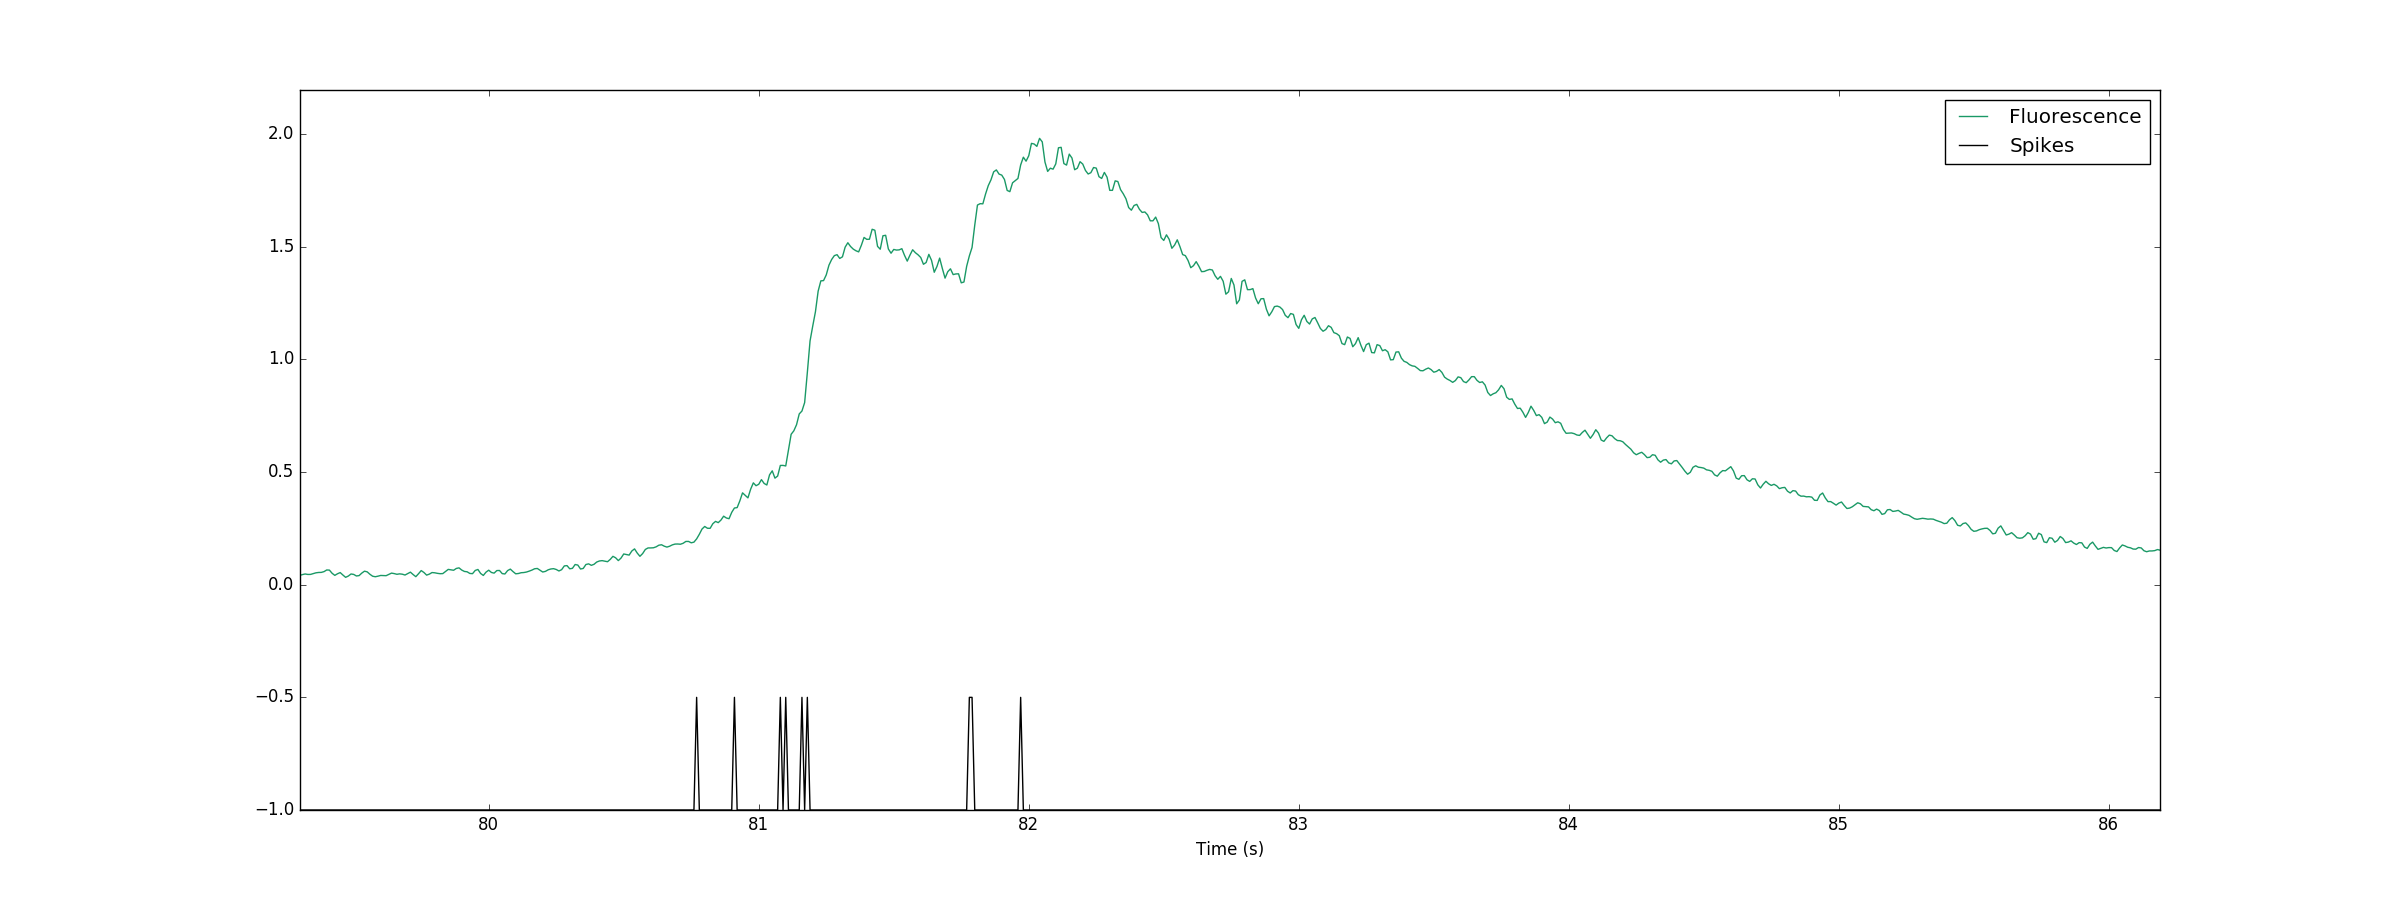
\includegraphics[width=\textwidth]{figures/zoomed_chen.png}
		\end{tabular}
		\caption{(a) Plot of a spike train and the corresponding GCaMP6s fluorescence trace. Data courtesy of spikefinder.codeneuro.org (b) The same image as (a) but zoomed into the period from 80s to 86s. A group of six action potentials around the 81s point followed by a group of three action potentials just before the 82s point are shown.}
		\label{fig:fluorescence_spikes}
	\end{figure}

	However, the dynamics of the fluorescent indicators are much slower than the dynamics of action potentials. After excitation the cross-membrane potential of a cell will return to baseline in $2-3$ms. After a single action potential, the fluorescence of GCaMP6s, one of the most popular calcium indicators, will return to baseline after approximately $3$s. At least a thousand times longer. An example of a fluorescence trace and the corresponding spike train is shown in figure \ref{fig:fluorescence_spikes}. Furthermore, the relaxation time is extended when more than one action potential is fired in quick succession \cite{chen}. It is claimed that despite this it is still possible to detect individual spikes even in spike bursts \cite{chen}, but I am not convinced. The GCaMP6s indicator is commonly used in the lab of Mike Ashby, who is my second supervisor. He has reported even longer relaxation times. Furthermore, readings are usually taken from cells after a `loading' period, so that the indicator is saturated within the cells. At this point the change in fluorescence in response to an action potential will be greatest. So another issue with the genetic indicators is that it is impossible to know whether or not the indicator is saturated within the cell. This is especially a problem with longitudinal studies, as the amplitude of fluorescence change in response to an action potential will change as the experiment goes on. This means that the same amount of activity in cells will cause different amounts of fluorescence changes at different times, which makes analysis difficult.
	
	There are existing methods for converting a fluorescence trace into a spike train \cite{paninski}, but these methods have not been tested rigorously. Also, these methods do not take variations in the concentration of the indicator into account. Furthermore, the process of collecting the photons emitted by the indicator introduces some noise. The amount of noise varies from indicator to indicator. Whether or not this noise is enough to obfuscate the spiking signal has never been investigated. A model of the fluorescence produced by a spike train is required to assess whether or not it is actually possible to extract an accurate spike train from a fluorescence trace. A model of this kind could also be used to test the methods that convert a fluorescence trace into a spike train. So I decided to build a model like this.
	
\subsection{Modelling}\label{modelling}
\subsubsection{Calcium dynamics}
	When a neuron fires an action potential this opens up voltage-dependent calcium ion channels, which allows a current of Ca$^{2+}$ to flow into the neuron \cite{koch}. This increases the calcium ion concentration [Ca$^{2+}$] inside of the cell. This, along with changes in the concentration of potassium and sodium, contributes to a change in the membrane potential which must be depolarised. The depolarising process consists of the free calcium ions leaving the cell through a molecular pump, leaving the cell through open ion channels, binding to molecules within the cell called \textit{buffers}, and some calcium storage by organelles such the endoplasmic reticulum. There are several different types of calcium ion buffer, each with different dynamics and different concentrations within different types of excitable cell. The fluorescent calcium indicator is another calcium buffer, with the useful property that when it is bound to a calcium ion, the bound molecule may become excited by a photon and release a photon in return. This is what creates the fluorescence. After the action potential has taken place, the free calcium concentration within the cell will return to a baseline level \cite{maravall}.

\subsubsection{The model} 
 	 I modelled the dynamics of five molecular concentrations within the body of a neuron, the free calcium [Ca$^{2+}$], the fluorescent calcium indicator [B], the endogenous calcium buffer [E], the immobile calcium buffer [Im], and the excited buffered calcium [BCa$^*$]. I initially modelled the dynamics using a \textit{piecewise-deterministic Markov process}, where the excitation and relaxation of the buffered calcium ions [BCa] was modelled using the Markov process, but I found this system too stiff with which to experiment. I then switched to a more traditional system of ordinary differential equations, with a stochastic photon collection model to introduce a source of noise. The chemical reactions governing the binding and unbinding of calcium from the different types of buffer are
	\begin{align*}
	[X][Ca^{2+}] \underset{b_X}{\overset{f_X}{\rightleftharpoons}} [XCa]
	\end{align*}	 	 
	where $[X]$ represents any one of the different kinds of buffer, and $f_X$ and $b_X$ represent binding and unbinding rates in units of per molar concentration per second ($M^{-1}s^{-1}$) and per second ($s^{-1}$) respectively. Ignoring the baseline level of calcium, the system of equations governing the model are as follows:
	\begin{align*}
	\diff{[Ca^{2+}]}{t} &= b_i [BCa] + b_E [ECa] + b_{Im}[ImCa] - f_i [B][Ca^{2+}]  \\ 
						&- f_E [E][Ca^{2+}] - f_{Im}[Im][Ca^{2+}] \\ 
	\diff{[BCa]}{t} &= f_i [B][Ca^{2+}] - b_i [BCa] + r[BCa^*] - e[BCa] \\ 
	\diff{[ECa]}{t} &= f_E [E][Ca^{2+}] - b_E [ECa] \\ 
	\diff{[ECa]}{t} &= f_E [E][Ca^{2+}] - b_E [ECa] \\
	\diff{[ImCa]}{t} &= f_{Im} [Im][Ca^{2+}] - b_{Im} [ImCa] \\ 
	\diff{[BCa*]}{t} &= e[BCa] - r[BCa^*] 
	\end{align*}
	where $e$ is the rate of excitation for the calcium ions buffered by the fluorescent buffer, and $r$ is the rate of photon release for those excited buffered calcium molecules. An action potential is simulated by setting the concentration of Ca$^{2+}$ within the neuron to an appropriate level \cite{maravall}.	The endogenous buffer and the immobile buffer are included to simulate the action of all the endogenous and immobile buffers collectively. The final goal of the model is to allow the parameters of all the buffers to be set, and an arbitrary spike train to be fed into the simulation, then the model will produce the corresponding fluorescence trace. Then the model can be used to assess the quality of the methods used to convert a fluorescence trace into a spike train, and it can be used to assess whether or not a conversion from fluorescence to spike train is possible.

\subsection{Results so far and future developments}
	At this point, the model can produce a fluorescence trace given an arbitrary spike train. The number of input parameters give the model a lot of flexibility. But the flexibility of the model has not yet been explored. At the moment I am aiming towards simulating GCaMP6s fluorescence traces accurately, and then moving on to trying to simulate the traces produced by other fluorescence traces. This part of the project will have ended after I have used the model to assess the accuracy of some fluorescence trace deconvolution methods. A possibility for extra work on this part of the project would be to develop an analysis method that measures how accurately a spike train can be recreated given the fluorescence trace produced by the spike train. The model would come in useful here as the level of noise in the fluorescence trace can be varied easily using the model. The accuracy of the fluorescence trace conversion method could be assessed as a function of noise. Another possible expansion on this work would be to use a number of existing spike trains and corresponding fluorescence traces to train the model for a particular fluorescence indicator.
	
	I have submitted a poster abstract to the BNA event in April on this research that has been accepted. It is under consideration for a short talk.

\section{Modelling the responses of populations of neurons}

\subsection{Developments in modelling of this kind}
	Before the mid-2000s much of what was known of neurons had been learned by either studying individual neurons or studying correlations between them \cite{zohary}. Extending these studies to larger populations of neurons had proven difficult. The main difficulty lay in the huge number of possible response patterns. In a population of $N$ neurons, there are $2^N$ possible response patterns for every time step. Building a model that specified a probability for each possible pattern in a population with $\sim 100$ neurons seemed impossible. The only way around this problem is to make some lower order approximations. Schneidman et al, (Nature, 2006) made a leap forward in this area when they applied a maximum entropy model equivalent to the Ising model to neuronal populations.
	
\subsubsection{Maximum entropy models}
	In a population of $N$ neurons, let $x_n$ represent the response of the $n$\upperth  neuron where $x_n \in \lbrace 0,1 \rbrace$ or $x_n \in \lbrace -1,1 \rbrace$, $n \in \lbrace 1, \dots, N \rbrace$. A zero or negative one corresponds to a resting neuron and a one corresponds to the firing of an action potential. The response of the population can be represented as a random variable $X$ that can take up to $2^N$ possible values or outcomes, and has a probability distribution $P(\mathbf{x})$. 
	
	The entropy of a random variable $X$, with outcomes $x_1, \dots, x_N$, and corresponding probabilities $p_1, \dots, p_N$ is defined as 
	\begin{align}
	H(X) = -\sum_{n=1}^N p_n \log _2 p_n \label{entropy}
	\end{align}
	This quantity is also known as the information entropy or the `surprise'. It was defined to express the amount of uncertainty in a random variable. For example, a variable with a probability of $1$ for one outcome, and zero for all others will have 0 entropy, because it contains no uncertainty. But a variable with a uniform distribution will have maximal entropy as it is the least predictable. this quantity is analogous to the entropy of a physical system \cite{shannon}. Note that any base may be used for the logarithm in equation \ref{entropy}, but using base two means that the quantity will be measured in units of bits.
	
	A maximum entropy model for a population of neurons is a model that defines the probability distribution, $P(\mathbf{x})$ that maximises the entropy of the population response under some constraints. The entropy of the population response is defined over the probabilities of each possible response pattern $\mathbf{x}$.
	\begin{align}
	H(X) = - \sum_{\lbrace \mathbf{x} \rbrace} P(\mathbf{x}) \log _2 P(\mathbf{x})
	\end{align}
	A maximum entropy distribution is usually found using the method of Lagrange multipliers \cite{jaynes}. Using this method ensures that no additional contraints are applied to the model other than those used to learn the parameters. Since it is clear that neuronal populations are strongly correlated and information is contained within those correlations \cite{zohary, schwartz}, it is common to include constraints on the correlations when learning a maximum entropy model. If we denote the probabilities of each possible pattern by $p_1, \dots, p_{2N}$, then when preserving all possible correlations, the Lagrangian takes the following form:
	\begin{align}
	\mathcal{L}(p_1, &\dots, p_{2N}, h_1, \dots, h_N, J_{12}, \dots, J_{N-1 N}, K_{123}, \dots) = \nonumber \\ 
	&H(p_1, \dots, p_{2N}) + \left(\sum_{n=1}^{2N} p_n - 1 \right) \nonumber \\ 
	&+ h_1(\langle x_1 \rangle - \mu_1) + \cdots + h_N(\langle x_N \rangle - \mu_N) \label{lagrangian} \\ 
	&+ J_{12}(\langle x_1 x_2 \rangle - \rho_{12}) + \cdots + J_{N-1 N} (\langle x_{N-1} x_N \rangle  - \rho_{N N-1}) \nonumber \\
	&+ K_{123}(\langle x_1 x_2 x_3 \rangle - \nu_{123}) + \cdots + K_{N-2 N-1 N}(\langle x_{N-2} x_{N-1} x_N \rangle - \nu_{N-2 N-1 N}) \nonumber \\
	&+ \cdots \nonumber
	\end{align}
	where $\mu_n$ is the observed firing rate of the $n$\upperth neuron of the population, $\rho_{n-1 n}$ is the pairwise correlation between the $n-1$\upperth and $n$\upperth neurons, $\nu_{n-2 n-1 n}$ is the three-way correlation between the $n-2$\upperth, $n-1$\upperth, and $n$\upperth neurons, and so on, and $h_n$, $J_{n-1 n}$, $K_{n-2 n-1 n}$, etc. are Lagragian multipliers. Learning a model from this Lagragian results in a probability distribution of the following form:
	\begin{align}
	P(\mathbf{x}) = \frac{1}{Z}\exp \left(\sum_{n=1}^N h_n x_n + \sum_{n<m} J_{nm} x_n x_m + \sum_{n<m<l}K_{nml}x_n x_m x_l \cdots \right) \label{distribution}
	\end{align}
	where $Z$ is the partition function \cite{schneidman_2003}. Note that for every order of correlations, there is a set of constraints on those correlations in equation \ref{lagrangian} and a sum in the exponential in equation \ref{distribution}. If no correlations are constrained, then $P(\mathbf{x}) = 1/Z$, which is a uniform distribution, and therefore maximises the entropy. If only the firing rates of each neuron are constrained, then $P(\mathbf{x}) = \frac{1}{Z}\exp \left(\sum_{n=1}^N h_n x_n\right)$. This is usually called the independent model, because it includes the (incorrect) assumption that all the neurons are independent.
	
	Including restrictions on all of the correlations is not realistic. This would require performing an experiment that yielded enough observations to estimate all of the correlation measures. With a population containing greater than $\sim20$ neurons, this is not possible due to the number of possible patterns $(2^{20})$. This explosion in the number of patterns to be observed, or the number of parameters to be estimated is often called the \textit{curse of dimensionality} \cite{schneidman_2006}. It is one of the reasons why computational/statistical modelling is so necessary for this area of neuroscience.
	
	So, not all correlations can be approximated in the model. The more correlations that are included, the more constrained the model will be, and therefore the lower the entropy of the model will be. Schneidman et al (Physical Review Letters, 2003) defined a measure for the amount of entropy contained in the correlations of a neuronal population, the multi-information. The multi-information is the difference between the entropy of the independent model and the entropy of the `true' distribution.
	\begin{align}
	I(\mathbf{x})^{(N)} = \sum_{n=1}^N H(x_n) - H(X)
	\end{align}
	Since not all correlations can be included, an interesting question is: how much of the multi-information can be captured by including only a small number of constraints. 

	Schneidman et al (Nature, 2006) answered this question and revolutionised the study of populations of neurons by applying a maximum entropy model \cite{schneidman_2006}. All of what is described above was known before this paper was written but, no one had thought of applying it to neuronal populations until this paper. 
	
	In the paper, the process outlined above was used to create a model which included the constraints on the pairwise correlations in the neuronal population. The resulting model took the form
	\begin{align}
	P(\mathbf{x}) = \frac{1}{Z}\exp \left( \sum_{n=1}^N h_n x_n + \sum_{n<m} J_{nm} x_n x_m \right)
	\end{align}
	Since the authors chose to have $x_n \in \lbrace -1, 1 \rbrace$, the resulting model was equivalent to the Ising model. The entropy of a model which preserves pairwise correlations is often denoted by $H_2(X)$, because correlations of the second order are preserved. Using this notation a quantity which measures the amount of entropy contained in the pairwise correlations was defined similarly to the multi-information
	\begin{align}
	I(\mathbf{x})^{(2)} = \sum_{n=1}^N H(x_n) - H_2(X)
	\end{align}
	The fraction of the multi-information contained in this `pairwise information' was measured, and found to be $\sim 90\%$. This result was reproduced using different stimuli and populations from different subjects. This meant that most of the information carried in the network correlations could be reproduced in a model by just preserving the pairwise correlations. It also meant that modelling the weak pairwise correlations in the neuronal population forced stronger correlations to arise. 
	
	This paper was not only significant because of the mulit-information result, but also because it showed that it was possible to model a population of neurons in a way that gave a full probability distribution for all possible patterns. Unfortunately, this model is only tractable for small populations ($N < 20$). This is because the number of parameters required scales with $N^2$ and also because the larger the population the more data is required to train the model. The pairwise maximum entropy model also seems to break down when applied to larger populations, implying that higher order correlations are more important in larger populations \cite{schwartz}. In particular the pairwise maximum entropy model appears to breakdown more for natural stimuli in comparison to artificial stimuli like spatiotemporal white noise \cite{ganmor}. Also, this model doesn't attempt to take into account the temporal correlations in neural data. This indicates that higher order correlations may be necessary to encode natural stimuli. A number of models were inspired by this paper, and attempted to improve upon it.
	
	One of the models inspired by the pairwise maximum entropy model was a pairwise spatio-temporal maximum entropy model \cite{marre}. This was constructed in a similar way, but with an additional constraint on $\langle x_n(t) x_m(t+1) \rangle$, and a marginal distribution constraint $\sum_{\mathbf{x}^\prime} P(\mathbf{x}^{\tau + 1}; \mathbf{x}^\prime) = P(\mathbf{x}^{\tau + 1})$ applied after using the method of Langragian multipliers to learn the parameters. It was also assumed that the transition between time steps behaved like a first order Markov process.
	
	The Markov model showed an improvement on the pairwise maximum entropy model when trained on synthetic data, and experimental data. The Shannon-Jensen divergence between the true distribution and Markov model was consistently an order of magnitude smaller than the divergence between the true distribution and the pairwise maximum entropy model. However, the Markov model has even more parameters to learn than the pairwise maximum entropy model. So although the problem of including temporal correlations is improved, all of the other problems of the pairwise maximum entropy model are present in the Markov model.
	
	A more recent and interesting maximum entropy model is described in \cite{gardella}. This model is inspired by the work done in \cite{okun} on population coupling. That study showed that each neuron in a population is influenced by the population rate, i.e. the number of neurons firing at any one time.
	\begin{align*}
	K = \sum_{n=1}^N x_n
	\end{align*}		
	So in \cite{gardella} Gardella et al chose to constrain the individual firing rates $\langle x_n \rangle$, the distribution of the population rate $P(K)$, and the linear coupling between the firing rates and the population rate $\langle K\cdot x_n \rangle$. They called this model the \textit{linear-coupling model}. They also went one step further and constrained the joint probability distribution of each neuron and the population rate $P(x_n, K)$. They called this model the \textit{complete-coupling model}. They compared these models to a simpler model created by only applying constraints to the firing rates and population rates called the \textit{minimal model}. 
	
	They found that each model could be written down as 
	\begin{align}
	P(\mathbf{x}) = \frac{1}{Z} \exp \left( \sum_{n=1}^N h_{n,K} x_n \right)
	\end{align}		
	where $n = 1, \dots, N$ and $K = 0, \dots, N$, with $h_{n,K}$ taking a different form for each model. For the minimal model $h_{n,K} = \alpha_n + \beta_K$. For the linear-coupling model $h_{n,K} = \alpha_n + \beta_K + \gamma_i K$. For the complete-coupling model $h_{n,K}$ is not restricted to any simpler formulation.
	
	The most attractive feature of either the linear-coupling model or the complete-coupling model is that they are tractable even when applied to large populations of neurons. This is because the partition function $Z$ can be broken down into a different partition function for each value of $K$, $Z_K$, which is equal to the $K$\upperth order coefficient of the polynomial
	\begin{align}
	Q(X) = \prod_{n=1}^N (1 + Xe^{h_{n, K}})
	\end{align}
	This allows $Z_K$ to be calculated in time linear in $kN$. The statistics of the model can then found using partial derivatives of the partition function. For example, the joint distribution of $x_n$ and $K$ is 
	\begin{align}
	P(x_n = 1, K) = \pdiff{\log Z}{h_{n,K}}
	\end{align}
	
	In addition to this, both coupled models showed great improvements over the minimal model in preserving pairwise correlations. This preservation was measured using a goodness-of-fit index. But the complete-coupling model showed only a small improvement over the linear-coupling model in this regard.
	
	The multi-information of both of the coupled models or the `coupled information' was also measured, and compared to the true multi-information. Smaller populations ($N=20$) had to be used for this as it is impossible to enumerate all of the possible patterns for a large population. It was found that the linear-coupling model captured 56\% of the multi-information, and the complete-coupling model captured 68\% of the multi-information. This is less than the 90\% captured by the pairwise maximum entropy model, but that model uses far more parameters, and is not tractable for large populations. The pairwise maximum entropy model also fails to capture the probability of patterns with large population rates \cite{tkacik}, which is captured by the coupled models. 
	
\subsubsection{Other types of models}
	Not all models are necessarily maximum entropy. The \textit{reliable interaction model} \cite{ganmor} is an example of a model that does not maximise the entropy. But it is based on the maximum entropy principle. It was observed that if $x_n \in \lbrace 1, 0 \rbrace$, then parameters in equation \ref{distribution} could be estimated directly from the experimental data using the set of linear equations
	\begin{align*}
	Z &= \frac{1}{P(\mathbf{x} = (0\dots0))} \\
	h_1 &= \log P(\mathbf{x} = (10\dots0)) + \log Z	\\
	J_{12} &= \log P(\mathbf{x} = (110\dots0)) + \log Z - h_1 - h_2 \\
	K_{123} &= \log P(\mathbf{x} = (1110\dots0)) + \log Z - h_1 - h_2 - h_3 - J_{12} - J_{13}- J_{23} \\
	 &\vdots
	\end{align*}
	The most frequently occurring patterns were used to estimate the parameters of the interactions governing the joint activity of the population and to build the model. Which patterns occurred sufficiently frequently was decided by choosing a threshold number of times that a pattern must occur before being used, denoted by $n_{RI}$. The model is designed this way in order to include higher order correlations which were not directly included in the pairwise maximum entropy model, and also to reduce the number of parameters that must be learned in order to implement the model. 
	
	The model succeeds in both of those objectives, and shows an improvement on the pairwise maximum entropy model particularly in modelling those patterns observed less frequently. Correlations of the third, fourth, and fifth order were used in the model, and it was shown that groups of neurons which showed the strongest correlations were usually close to one another. Significantly fewer parameters were required for the reliable interaction model in comparison to the pairwise maximum entropy model. The reliable interaction model used 450 parameters to model 99 neurons. The pairwise interaction model would need 4950 parameters to model this many neurons. 
	
	A major drawback of the reliable interaction model is that it does not return a normalised probability distribution over the possible patterns. The pairwise maximum entropy model does achieve this for small populations only. Without this property, the reliable interaction model cannot give a probability for a given firing pattern. Any model which aims to improve on the pairwise maximum entropy model should retain this property. It would be possible to fix this problem by using an `estimator' to assign probabilities to the unobserved patterns. Examples of possible estimators that could be used are the `singleton' estimator and `coverage adjusted' estimators. I have proposed to do this as a summer school project in the OCNC course in computational neuroscience this summer. I do not know if I have been chosen to attend this conference yet. 
	
	Another drawback of the reliable interaction model, which it shares with the pairwise maximum entropy model is that it only takes into account spatial correlations, even though it is known that temporal correlations hold information about the stimulus \cite{schwartz}.
	
	Another model that has not been proven to be a maximum entropy model (but claims to be) is the population tracking model by my supervisor Dr. Cian O'Donnell \cite{odonnell}. Like the maximum entropy population coupled model in \cite{gardella}, this model was also inspired by the work done by Okun et al in \cite{okun}. The model preserves the population rate distribution, $P(K)$, and the conditional firing rate of each neuron in the population, conditioned on the population rate, $P(x_n | K)$. The model assumes that the neurons are conditionally independent given the population rate, so it gives the distribution
	\begin{align}
	P(\mathbf{x}) = \frac{P(K)\prod_{n=1}^N P(x_n | K)^{x_n}(1 - P(x_n | K))^{1-x_n}}{a_K}
	\end{align} 
	where $a_K$ is a normalizing constant to correct for the fact that if neurons were truly conditionally independent given a population rate of K we could not guarantee that we would have exactly K of them active.
	
	After fitting the model to a data set, the model manages to reproduce the firing rates of each neuron observed in the data. It also manages to reproduce the pairwise correlations to an extent. The mean pairwise correlation is preserved, but the finer features of the pairwise correlations are not. As with a number of models for neuronal populations, this model does not preserve the temporal correlations because it is not designed to do so.
	
	Another common feature between this population tracking model and \cite{gardella} is the tractability of the model. This is a massive attraction as it allows the model to give a fully normalised probability distribution across all possible patterns, which was one of the main aims of the model when it was designed. This model is tractable because the parameters are very easy to estimate. The probability distribution of the population rate $P(K)$ can be estimated using simple histogramming. This gives the \textit{maximum likelihood estimate} of the probabilities. This combined with regularization using a Bayesian prior to avoid naively assigning zero probability to unobserved population rates gives the \textit{maximum a priori} estimate of these parameters. Use of a Dirichlet prior gives the expression
	\begin{align}
	P(K, \alpha) = \frac{c_K + \alpha}{T + N\alpha}
	\end{align}
	where $c_K$ is the number of time-points observed where $K$ neurons are active, and $T$ is the total number of time-points. The $\alpha$ hyperparameter is a small positive constant corresponding to a pseudo-count. 
	
	The conditional probabilities can be estimated in a similar way. Again histogramming is used and combined with a Beta prior distribution to give a MAP estimate of
	\begin{align}
	P(x_n | K, \beta_0, \beta_1) = \frac{d_{n,K} + \beta_1}{\beta_0 + \beta_1 + T_K}
	\end{align}
	where $d_{n,K}$ is the number of times that the $n$\upperth neuron fired an action potential when the population rate was equal to $K$, $\beta_0$ and $\beta_1$ are the parameters of the Beta distribution, and therefore the hyperparameters of the conditional distribution. These are set in accordance with the mean and variance of a Bernoulli distribution with `on-probability' $\frac{K}{N}$. Alternatively, logistic regression could be used to fit these parameters. But this approach was found to give inferior fits \cite{odonnell}.
	
	In comparison to the model of Gardella et al, this model suffers from not being proven to be a maximum entropy model, but the author's conjecture that the model is a maximum entropy model is easy to believe. This population tracking model also assumes that the neurons are conditionally independent given the population rate, which is not true. The linear-coupling model makes the same assumption, but the complete-coupling model does not. On the other hand, the parameters of the coupled models are learned using Newton's method. O'Donnell's method for fitting the parameters is easier to implement. 
	
		
\subsection{Plans for future research}
	In the sections above I have outlined a number of methods for estimating the pattern probability distribution of a population of neurons. But I have given no examples of how these models can be used to address a particular question in neuroscience. Coincidentally, the question of how the representation of stimuli changes during brain development in healthy and diseased subjects has yet to be answered and requires some research. I aim to either develop a new modelling method or augment an existing one in order to address this issue.

	There are three main objectives to my research. The first objective, the calcium fluorescence modelling, is only tangentially related to the last two objectives. But because the calcium fluorescence modelling is required by the research community, and it could be completed within a few months, I plan to finish up this part of the project while I continue to familiarise myself with the modelling of neuronal populations.
	
	So the first part of my research is to develop a model of the fluorescence produced in the soma of a neuron that expresses a calcium sensitive fluorescent protein, during a spike train. See section \ref{modelling} for details. 
	
	The second objective will be to develop a method of modelling a large population of neurons that encompasses some parameter(s), which enable a comparison of internal representations of a stimulus, or stimuli, across different stages of development. At the moment, in order to compare the representation of a stimulus at different times, it is necessary to model the representation at each time point as though the models are independent of one another. This assumption of independence must necessarily throw away some mutual information between the two representations. Developing a model like the one described will enable some interpolation along the temporal parameter(s), and will give some insight into how this information is retained by the population. Initially, an existing model such as Cian's population tracking model can be extended, including the age of the subject as a parameter. Once some analysis has been completed, the question of which parameters to add will readdressed. A secondary affect of this research will be that it could give some insight into how the temporal correlations between response patterns could be modelled. As I mentioned above, the spatial correlations between individual neurons, or between neurons and their population are usually used for modelling, but the temporal correlations are often ignored.
	
	The final objective is to use this model to analyse the differences in development between healthy subjects, and subjects with a neural disorder, for example mice with dementia. The model developed in the second objective will allow the differences between the two types of subjects to be quantified. The healthy subjects can act as a control group for the test subjects. The data for this study will come from Mike Ashby's lab. Mike is my second supervisor and has said that he will be able to provide data over multiple time points from healthy mice and mice engineered with a tauopathy. The brain region to be studied will be mouse somatosensory (or barrel) cortex as this part of the cortex is connected to the mouse's whiskers, so it is easy to stimulate, and some of the structure of these connections is known. The activity of this brain region will be monitored using an expressed fluorescent calcium indicator. So the first objective of the project will be useful in this context. Quantifying the differences between development points and subjects will consist of constructing the model at those different points and in those different subjects and doing some interpolation along the temporal parameter(s). The traditional approach of using some analytic such as the Kullback-Leibler divergence or the Shannon-Jensen divergence to measure the difference between the two will also be taken. Other functions of the pattern probability distribution like the entropy, or the mutual information between the response and the stimulus will also be worth measuring. Statistics of the individual neurons such their firing rates and their cross correlations will also be useful.

	The affects of my research will be to address the question of representational changes in brain development directly and to develop an analysis method that includes some temporal structure. The temporal part of the model will be longitudinal in neuroscience terms, and therefore will not be directly relevant to the issue of temporal correlations between firing patterns. But it will uncover an approach which will be applicable to this problem.

\newpage
\bibliography{./six_month_report.bbl}

\end{document}